\documentclass[oribibl]{llncs}
\usepackage{graphicx}
\usepackage{amsmath}
\usepackage{textcomp}       % additional symbols using companion encoding TS1
\usepackage{epstopdf}
\usepackage{nameref}

\title{Collabot}
\subtitle{A Collaborative Robotic Agent for the CiberRato Competition - Mapping and Communication}
\author{H\'{e}lder Moreira \and Tiago Babo}
\institute{Faculdade de Engenharia da Universidade do Porto}

%
\begin{document}
\maketitle
\begin{abstract}
This paper discusses the implementation of mapping and communication for a collaborative robotic agent, using the Ciber-Rato Simulation Tools. Navigation and target localization strategies were also implemented in the discussed agent, however those implementations are further explained in the paper by Pontes and Varela \cite{varelaepontes}.
We focused on developing an interesting solution for a maze solver agent and explore the collaboration between robots with similar architectures.
\end{abstract}

\section{Introduction}
Ciber-Rato is a category of the Micro-Rato contest from University of Aveiro.
This category is a competition between small autonomous robots trying to solve mazes \cite{Lau2002}. 
In this project, we faced the challenge of developing a collaborative robotic agent architecture using the Simulation Tools created for the Ciber-Rato competition. The agents should be able to solve simple mazes by finding a beacon and returning to their original position, while avoiding obstacles, collisions and dealing with time constraints. Furthermore, in the collaborative competition, the agents are playing in a team of 5 robots, all the robots must meet in the target area and after that return to their original position. The maze is only considered solved when all the mice return to their original position.

At the starting point, the agents have no previous information about the world state, namely the target position, maze's topology and even his or other mice positions. Therefore, a simple reactive robot architecture was not suitable for this problem, so proper communication, mapping, navigation and target localization strategies were be developed in order to maximize the agent's efficiency.

In this paper, first we present the simulation system architecture. Then the agent architecture and design are analyzed, mainly focusing in the mapping and communication strategies, since navigation and target localization strategies are further discussed in the paper by Pontes and Varela \cite{varelaepontes}. After that, the results of the developed strategies are discussed. Finally, in the last section, are presented the main conclusions and some possible future developments.

\section{Simulation System Architecture}
To develop this project the Ciber-Rato Simulation Tools, 2012 edition, were chosen as a simulation platform. This platform allows the developers to focus only on the development of an efficient agent algorithm, eliminating the problems and challenges associated with real robots construction by providing a simulation environment that models all the hardware components of the robots and a allows the developed algorithms to be tested \cite{Lau2002}. 

The simulation environment is composed by a Simulator, a Simulation Viewer and Virtual Robots. The first is responsible for modeling all the hardware components of the robots, the maze and ensure that all the execution rules are applied. The Simulation Viewer displays the maze, the robots movements and the remaining execution time. The virtual Robots are detailed in the section bellow.

All the specifications presents in this paper are based on the Ciber-Rato 2011 Rules and Technical Specifications \cite{DepartamentodeElectronica2011}, and only a brief specification is present in here, for a more detailed specification please consult the document mentioned above.

\subsection{Virtual Robots}
The virtual robots have circular bodies and are equipped with sensors, actuators and command buttons. Only the robots' sensors and actuators used by the agent that we developed are mentioned in this section.

\subsubsection{Sensors}\hfill \\
For the developed agent the following sensors were used, from the ones available in the simulation environment: 
\begin{itemize}
  \item[\textbf{Obstacle Sensors}]
  4 proximity sensors, 3 oriented to the front of the robot (left, middle and right sides), and one in the rear. Each sensor has a $60^{\circ}$ aperture angle.
  \item[\textbf{Beacon Sensor}]
  Measures the angular position of the beacon with respect to the robot's frontal axis. The measure ranges from $-180$ to $+180$ degrees, with a resolution of 1 degree.
  \item[\textbf{Bumper}]Active when the robot collides.
  \item[\textbf{Ground Sensor}]
  Active when the robot is completely in target area.
  \item[\textbf{Compass}]
  Positioned in the center of the robot and measures its angular position with respect to
the virtual North ($x$ axis).
  \item[\textbf{GPS}]
  Returns the position of the robot in the arena, with resolution 0.1. It is located in the center of the robot.
\end{itemize}

\subsubsection{Actuators}\hfill \\
The actuators components of the robots used in this project are 2 motors and 1 signaling LED. 
\begin{itemize}
  \item[\textbf{Motors}]
Motors have inertia and noise in order to more closely represent real motors, and the translation or rotation movements can be achieved by applying different power values to each motor.
  \item[\textbf{LED}]
The LED is used to signal that the robot has already found the beacon.
\end{itemize}

\subsubsection{Buttons}\hfill \\
Two buttons, named Start and Stop, are provided in each robot and are used by the simulator to start and interrupt the competition.

\subsection{Arena}
The arena is randomly positioned in the world, which means that the starting coordinates of the robot may differ for every attempt to solve the maze, and has a maximum size of $14\times28$ um.
The arena is populated with obstacles, a target area, and a starting grid. For the same maze different starting grids can also be used. The obstacles within the arena can be higher then the beacon, making it invisible for the beacon sensor.

\subsection{Communication}
Communication between robots can be made by sending appropriate commands, through the Simulator. The other agents will be then responsible for reading the messages in the simulator. However the following constraints are be applied:
\begin{itemize}
 \item Per cycle, a robot can send (broadcast) up to 100 bytes;
 \item Per cycle, a robot can read up to 400 bytes;
 \item Robots can only read messages sent from a maximum of 8 units from its current position;
 \item Obstacles do not interfere with communication;
 \item Latency of 1 cycle for sent messages.
 \end{itemize} 

\section{Agent Architecture}
In this project we faced the challenge of creating a team of 5 robotic agents, playing simultaneously, in the environment provided by the Ciber-Rato Simulation Tools.
The Mice have two specific goals: locate the target area and place all the agents inside that area; return all the robots back to their original position.

In order to achieve that goal our agents must be able to fully operate in an unstructured environment by avoiding obstacles and finding the beacon in a simple to moderately complex map. 
However, at the starting point, the agents have no previous information about the world state, namely the target position, maze's topology and even his or other mice positions. Therefore, a simple reactive robot architecture was not suitable for this problem and so proper communication, mapping, navigation and target localization strategies were be developed in order to maximize the agents efficiency.

The developed agent architecture is composed by 5 different modules and is represented in figure \ref{fig:robot-arch}.

\begin{figure}
  \centering
  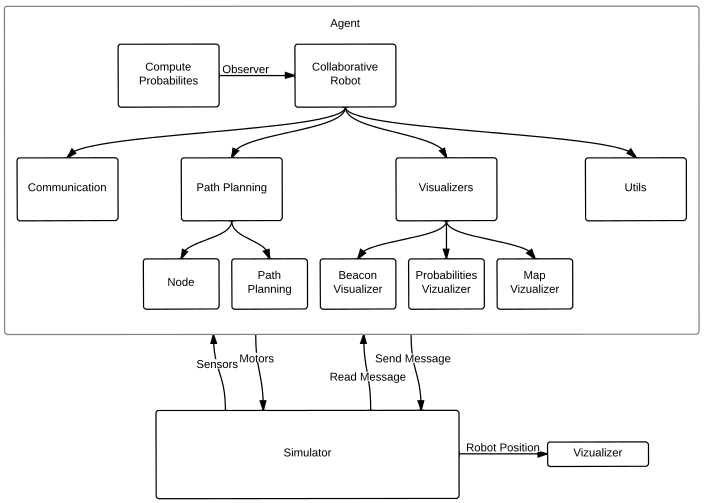
\includegraphics[width=0.9\textwidth]{robot-architecture.png}
  \caption{System architecture.}
  \label{fig:robot-arch}
\end{figure}

Bellow, the description of each module:

\begin{itemize}
  \item[\textbf{Compute Probabilities}]
  An observer that receives information from the sensors and updates the agent’s wall probability matrix.
  \item[\textbf{Communication}]
  Handles the communication betweeen the agent and the simulator, sending and receiving messages and updating the agent's knowledge accordingly. 
  \item[\textbf{Path Planning}]
  Traces the way back to the starting position after the agent reaches the objective.
  \item[\textbf{Visualizers}]
  Responsible for the visualizers that show the robot's internal information.
  \item[\textbf{Utils}]
  Used to store some constrained parameters, like arena size, map precision and other settings values.
\end{itemize}

\subsection{Mapping}

As previously mentioned, the map arena has a maximum size of 14 x 28 um and the simulator has a precision of 0.1 um. Considering that the initial position of the agent is not initial known, it was necessary to quadruplicate the structure where the arena is mapped. Doing this, it is possible to predict the agent movement in any direction. It was also considered the minimum value of precision, resulting in a matrix of 280 x 560 positions. 

Given that the agent has three sensors that allow him to detect, with noise, obstacles in the environment and that is only known that there is an obstacle in a given distance, it is not possible to have completely certainty about the obstacles position. The values provided by the sensors follow an additive white Gaussian noise deviation of 0.1 and they are the inverse to the distance of the closest obstacle detected. In order to minimize this constraint, the arena is mapped using a probabilities matrix. At start, the arena is not yet explored, hence all positions of the matrix have a probability of being an obstacle of 0.5.  

As the agent moves, the probabilities matrix is updated with new values, allowing to visualize and create a close to reality arena representation. To better use the sensor values, the area represented by the read values is divided in three sections. This implementation use the same approach of YAM \cite{Ribeiro2002}.

\begin{figure}
  \centering
  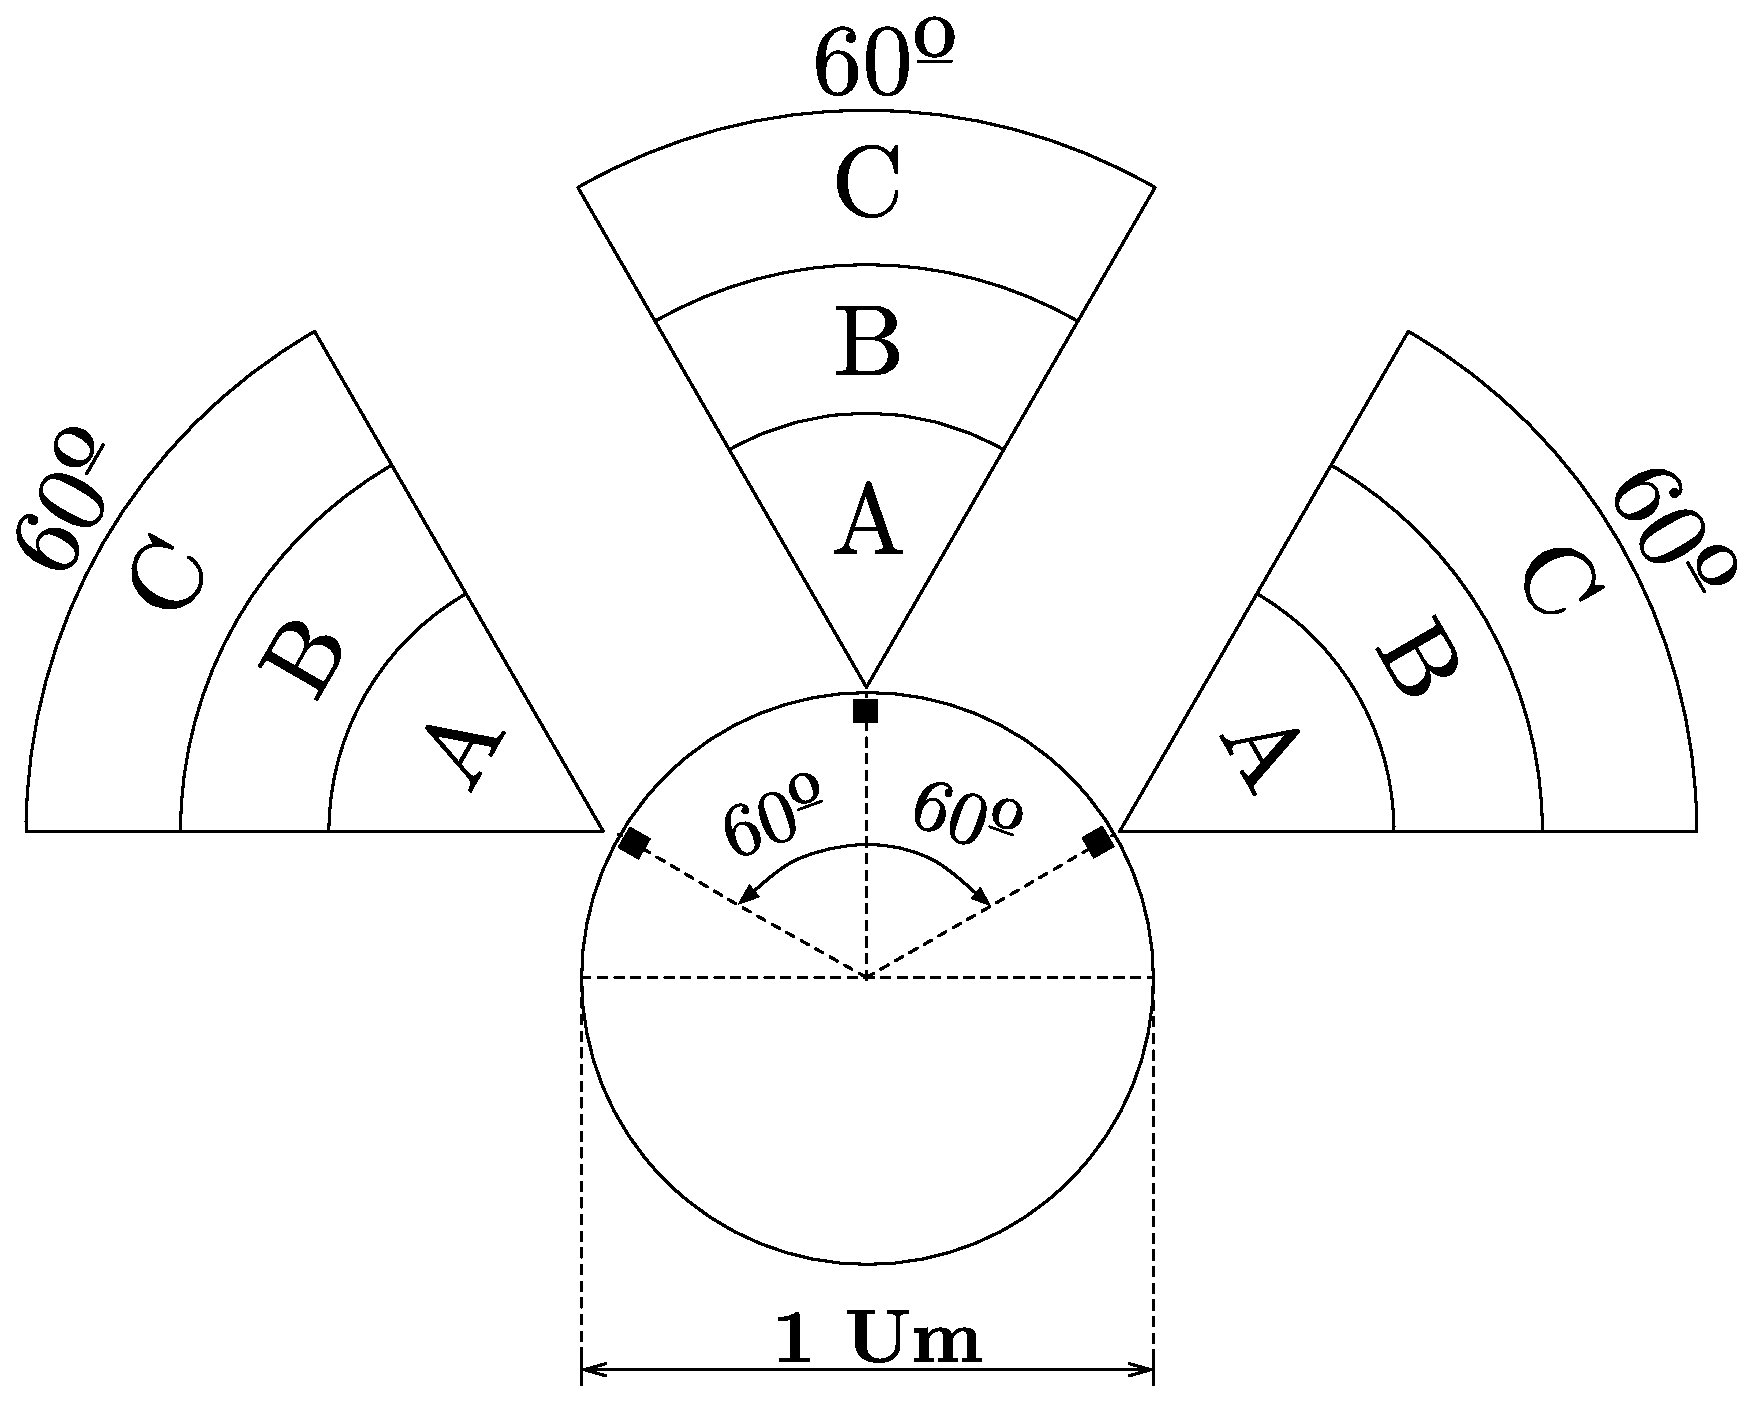
\includegraphics[scale=.25]{sensorareas.eps}
  \caption{Sensor areas.}
  \label{fig:sensorareas}
\end{figure}

\begin{itemize}
  \item[\textbf{A}]
  The area up to $\dfrac{1}{reading + noise}$ is marked has having a low probability of being a wall.
  \item[\textbf{B}]
The area up to $\dfrac{1}{reading} - wall width$ is marked has having a moderate probability of being a wall.
  \item[\textbf{C}]
  The area up to $\dfrac{1}{reading} + wall width$ is marked has having a high probability of being a wall.
\end{itemize}

Furthermore, when the agent is moving, the positions where he passes have zero probability of being a wall, so they are marked accordingly with that rule. 

As the positions have already a probability value, at every instant \emph{t} the probability of each affected position \emph{(i, j)} - as in, in the sensor area - is updated using the Bayes theorem rule:

 \begin{equation}
     P_{ij}(H|s_n) =   \dfrac{P_{ij}(s_n|H). P_{ij}(H|s_{n-1})}{P_{ij}(s_n|H).P_{ij}(H|s_{n-1})+ P_{ij}(s_n|~H).P_{ij}(~H|s_{n-1})}
\end{equation}

 $P_{ij}(H|s_n)$ is the probability of the \emph{(i,j)} cell being occupied given a certain measure $s_n$.

There are two conditions in order to a cell to be in the sensor area. First, the euclidean distance between the center and the given cell \emph{(ij)} has to be less than the inverse of the read value from the sensor plus the wall width. 

 \begin{equation}
    \sqrt{(X_{ij}-X_c)^2 + (Y_{ij}-Y_c)^2} < \dfrac{1}{reading} + wall width
\end{equation}

Second, the atan2 value, that represents the angle in radians between the positive x-axis of a plane and the point given by the coordinates (x, y) on it, has to be in the sensor vision angle range.

 \begin{equation}
    atan2(Y_{ij}-Y_c, X_{ij} - X_c) >= angleBegin \,\,\&\,\,\, atan2(Y_{ij}-Y_c, X_{ij} - X_c) <= angleEnd 
\end{equation}

If this two conditions are true, the cell probability is updated using the previous described method.

\section{Communication}
\label{communication}

The communication between the robots is handled by the simulator, which receives the messages from the sender and is responsible for propagating it to all the other robots that are registered in it. 

While these messages allow the robots to share knowledge among them, there are some limitations as detailed previously. Each robot, per cycle, is only able to send messages up to 100 bytes and able to receive up to 400 bytes (one message from each one of the other four). Besides these size limitations, there are also constraints regarding the distance the robots need to be from each other to be able to share the messages, that being 8 distance units, and regarding the latency of the communication, which is of 1 cycle per message.

With these limitations and the importance that the communication takes in a collaborative scenario in mind, the task of choosing what information to send in the messages, and how to send it, was, without a doubt, challenging. In this robot we opted for a strategy where two types of messages are transmitted (alternating in each cycle) when the robots are within range: sensors messages and beacon messages.

\subsection{Sensors messages} \label{subsec:sensor_messages}

Sharing the information gathered so far from the external environment was one of the goals of the communication module, but given the message size limitations, and the fact that we represented the map with a precision of 10 (i.e. each unit of the real map is represented by 10 cells in our matrix), the (ideal) option of transmitting the entire matrix was discarded and we opted for an approach that sends the readings from the robot sensors and its position.

This approach allows the robot to "see" what the other robots are seeing, interpret that data  and map the environment in a more efficient way than compared to one where no information is transmitted.

Below we can see a template for the sensors message:

\begin{verbatim}

"sensors|x|offsetX|y|offsetY|frontsensor|leftsensor|rightsensor|compass"

\end{verbatim}

The values x and y represent the robot coordinates in the position matrix.

The values offsetY and offsetX represent the offset of the robot position, calculated with the aid of the GPS in the first cycle, and allow for the robots to establish the teammate position in their own map, which otherwise would be misleading since the arena is randomly positioned in a world, being the origin coordinates (the left, bottom corner) assigned a pair of values in the range 0 to 1000.

After that, the values of the sensors are passed, front sensor, left sensor, right sensor and compass, to allow the recipient robot to map the environment, the same way the sender robot would do.
Since these messages are sent from all the robots to all, given the necessary exchanges, the robots will share the same map, and be aware of areas that they may have not yet visited, improving the overall performance of the team.

\subsection{Beacon messages} \label{subsec:beacon_messages}

The beacon messages goal is to share with the rest of the team, the information about the beacon gathered so far. The limitations explained above were again an issue, and with that in mind we opted for a strategy where we calculate the area where it is most probable for the beacon to be and share that in a message with the following template:

\begin{verbatim}

"y-offsetY-x-offsetX-value|value;value;value|value..."

\end{verbatim}

The values x and y represent the robot coordinates in the position matrix.

The values offsetY and offsetX represent the offset of the robot position, as detailed in section \ref{subsec:sensor_messages}.

After that, the values from the area are passed, from the top left to the bottom right.
This allows for the robots to have information about the beacon even if they themselves haven't seen it and in a scenario where enough messages are transmitted, allows for the robots to perfect each other's matrices and map the beacon position much more efficiently.


\section{Results}

In order to evaluate the agent implementation, the developed solution was tested in different arenas and multiple times.

\subsection{Mapping}

The results showed that the mapping algorithm can create a good visualization of the world state, without consuming too much resources. The major problem encountered was in mapping corners as rounded - when the agent was far from them. This happens because the sensor area is interpreted has a semi-circular form. 

\begin{figure}
  \centering
  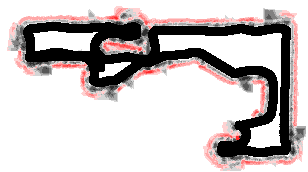
\includegraphics[width=0.6\textwidth]{screenmap.png}
  \caption{Partial mapping example. The red areas represent high probability of an obstacle and the black ones passable zones.}
  \label{fig:screenmap}
\end{figure}

As can be seen on figure \ref{fig:screenmap}, this model isn't perfect, but has a good effectiveness. The probabilities matrix is mainly used to calculate the path when returning home, after finding the beacon. The represented arena is on figure \ref{fig:originalmap}.

\begin{figure}
  \centering
  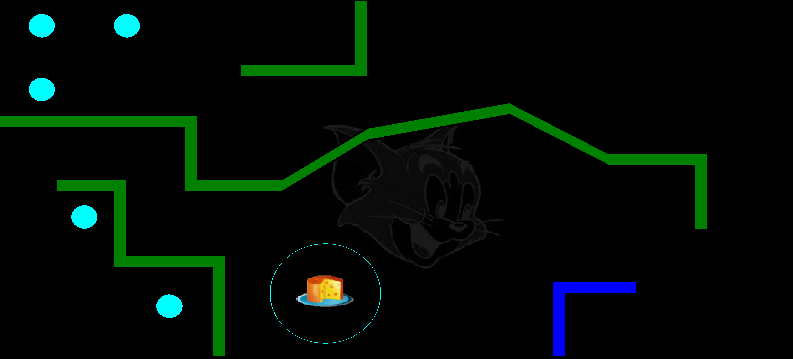
\includegraphics[width=0.8\textwidth]{originalmap.png}
  \caption{Original arena.}
  \label{fig:originalmap}
\end{figure}

\subsection{Communication}

As has been detailed in the \nameref{communication} chapter, the communication module introduces a way for robots to share their knowledge and improve the overall performance of the team.
In the following scenario, figure \ref{fig:viewer}, robot 1 doesn't receive any information related to the beacon due to it being blocked by an obstacle. On the other hand, robot 2 after a while starts to see the beacon in a straight line and gets also in a position where he can communicate with robot 1, making this the perfect scenario to test the communication module.

\begin{figure}
  \centering
  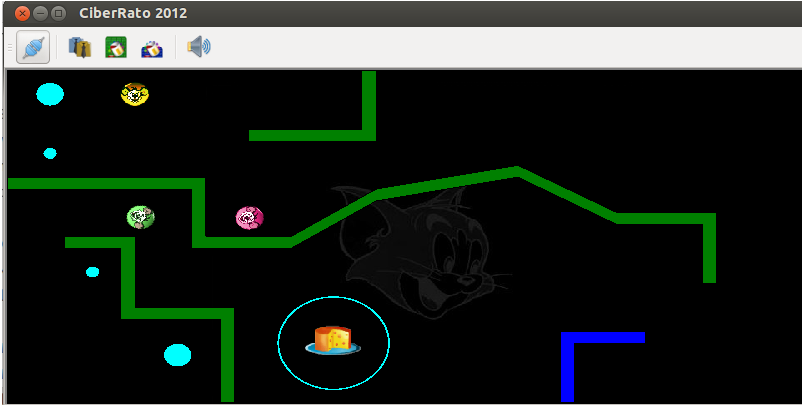
\includegraphics[width=0.8\textwidth]{viewer.png}
  \caption{Scenario where one of the robots has an obstacle blocking the beacon and the other is able to see it.}
  \label{fig:viewer}
\end{figure}

The following figures ( \ref{fig:visualizer1} and \ref{fig:visualizer2} ) represent each robot's knowledge about the beacon at that time. As can be seen, even though robot 1 is not able to receive the beacon sensor, he still gathers information about his target through communication with the robot 2, improving his performance.

\begin{figure}
  \centering
  
\includegraphics[width=0.8\textwidth]{visualizer1.png}
  \caption{Robot 1 beacon visualizer}
  \label{fig:visualizer1}
\end{figure}

\begin{figure}
  \centering
  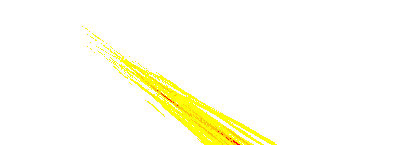
\includegraphics[width=0.8\textwidth]{visualizer2.png}
  \caption{Robot 2 beacon visualizer}
  \label{fig:visualizer2}
\end{figure}

\section{Conclusion and Future Work}

In general, the developed agent can solve different types of maps and return home with success. Although it has some problems avoiding some obstacles structures, the results were generally positive.

Regarding the mapping solution, the algorithm builds a good representation of the arena and produces good results that can be used later. As described in the paper by Varela and Pontes \cite{varelaepontes}, the probabilities matrix was used to calculate the path when returning home after some changes and considerations. In terms of improvements, it would be possible to improve corners detection, allowing a better arena representation.

As for the communication module, the approaches chosen have proven to improve the team's overall performance, allowing them to share information and knowledge about the external environment. Since the probabilities matrix is used mainly to calculate the return home path, and every robot will know at least one path home, we focused on sharing the beacon position knowledge to improve the performance in the first part of the competition. This way, improvements could be made to the sensors message, even though a functional version is implemented and working, to increase the amount of information transmitted, thus increasing the optimality of the return home path.


\bibliography{report}
\bibliographystyle{splncs}
\end{document}